\documentclass[a4paper,12pt]{article}
\usepackage{caption}
\usepackage{subcaption}
\usepackage{graphicx}
\graphicspath{ {img/} }
\usepackage{fancyhdr}
\pagestyle{fancy}
\lhead{tqvj24}
\chead{}
\rhead{Image Processing Assignment}

\begin{document}

\section*{Discussion and detail of system design and choices made}
\subsection*{System Design}
I used Python 3.5.2, and OpenCv 3.1.0, matching the versions available on the DUDE PCs in the School.
Key presses control the script, and output is shown in the main window, as well as various images being saved to disk, in the img\_out/ directory.
One file ID is displayed at a time, the top row being the w1 channel, and the bottom being w2. These are labelled, which can be toggled; see below.
Full list of commands:
\begin{itemize}
    \item n - next image
    \item b - previous image
    \item l - toggle labels
    \item s - save the current w1 and w2 processed images
    \item x - exit
\end{itemize}
There are settings under the imports, which enable automatic saving of various images.
\\\\
Processing of images is done in the following steps, where each step is a standalone, documented, and commented method.
\begin{enumerate}
    \item Isolate and compare
    \begin{enumerate}
        \item Isolate the worms from the background and border.
        \item Compare the isolated worms against the provided ground truth.
    \end{enumerate}

    \item Individualise and save each worm
    \begin{enumerate}
        \item Run the watershed algorithm to mark worms with unique colours.
        \item Save each individual worm, under img\_out/separated/ directory. This sub-step also prints the amount of worms counted.
    \end{enumerate}

    \item Label each worm either dead or alive
    \begin{enumerate}
        \item Find the rotated bounding box of each contour, and classify dead or alive depending on the width/height ratio of this box.
    \end{enumerate}
\end{enumerate}
Examples of what the above steps produce can be found under later sections. All images shown are of A01 w2, to clearly demonstrate the changes.

\subsection*{Choices Made}
As the images are saved as 16 bit but only actually using 12 bits, when reading as 8 bit images the 4 most significant bits were lost, and the image was very dark (Figure a), and so I read in the images as 16 bit, right shifted by 4 bits, and then converted to 8 bit. This ignores the 4 least significant bits, in favour of the 4 most significant bits. This results in a more usable, brighter image (Figure b).\\
\begin{figure}[ht!]
    \centering
    \begin{subfigure}{0.45\textwidth}
        \centering
        
\includegraphics[width=0.8\textwidth]{A01_step0_unshifted.jpg}
        \caption{Loaded as 8 bit}
    \end{subfigure}%
    \begin{subfigure}{0.45\textwidth}
        \centering
        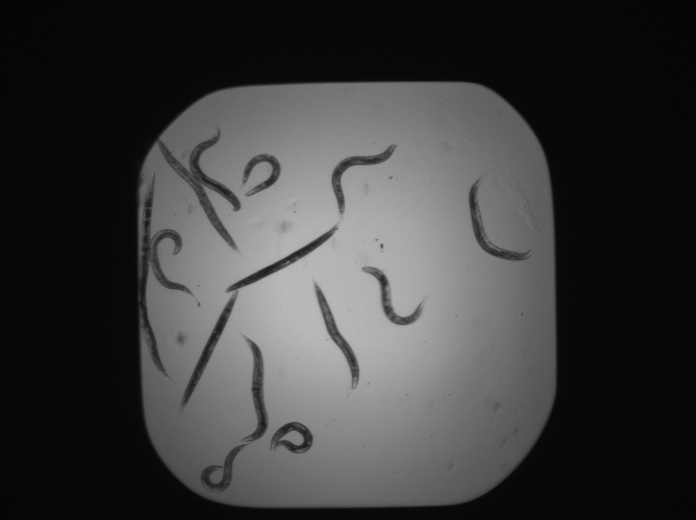
\includegraphics[width=0.8\textwidth]{A01_step0.jpg}
        \caption{Loaded as 16 bit and shifted}
    \end{subfigure}
\end{figure}
\\
I then adjusted brightness, and I found OpenCV's adaptive threshold to be much more effective than it's histogram equalisation, and the option to convert to a binary image proved useful.
\\\\
The next choice I made was border removal for w2. My initial attempt found all contours and filled the largest in black, assuming this was the border. This worked for most images, although big worm clusters occassionally had more area than the border, and so were removed instead. I instead settled on dilating a flood fill that started from the point (0, 0). This meant that it would surround the border, and slowly grow over it. Experimenting with the values given to this function resulted in excellent border removal.
\\\\
To compare my binary images to the ground truth, I simply subtract one from the other, causing discrepancies to show in white. This always results in high percentage values due to large empty spaces, however other methods seemed to always provide no measure of how good their result actually was, just numbers without context.
\\\\
For dead/alive classification, I initially tried checking contours with a method called isContourConvex, to indicate a curve/line. This method was not working well for this purpose, so I changed to checking the width/height ratio of rotated bounding boxes around worms.

\section*{Evidence of the success of the system in performing the specified tasks}
Figure 1: The loaded image, after shifting, before any major processing steps.\\
Figure 2: After step 1, worms isolated from the background and border.\\
Figure 3: After step 2, worms outlined in red.\\
Figure 4: After step 2 also, each worm marked a unique colour.\\
Figure 5: After step 3, worms coloured green if alive, red if dead, and boxed in purple.

\begin{figure}[ht!]
    \centering
    \begin{subfigure}{0.5\textwidth}
        \centering
        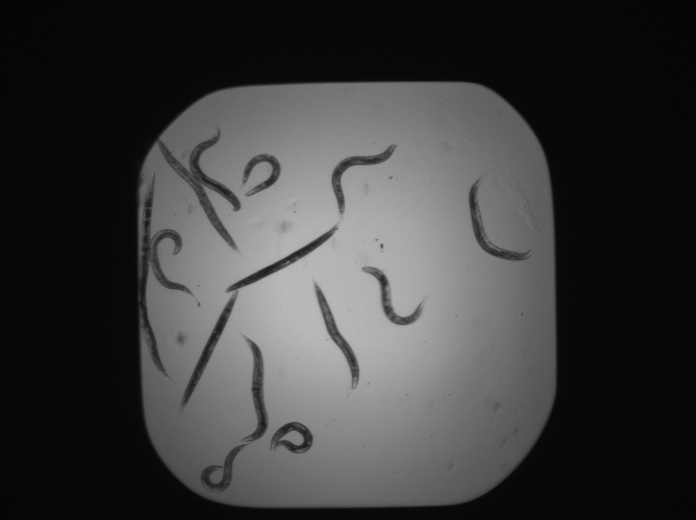
\includegraphics[width=0.9\textwidth]{A01_step0.jpg}
        \captionsetup{labelformat=empty}
        \caption{Figure 1}
    \end{subfigure}%
    \begin{subfigure}{0.5\textwidth}
        \centering
        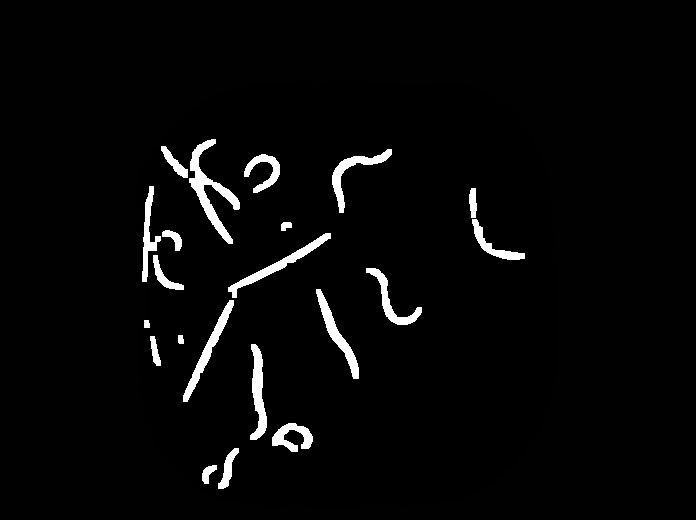
\includegraphics[width=0.9\textwidth]{A01_step1.jpg}
        \captionsetup{labelformat=empty}
        \caption{Figure 2}
    \end{subfigure}
\end{figure}
\begin{figure}[ht!]
    \begin{subfigure}{0.5\textwidth}
        \centering
        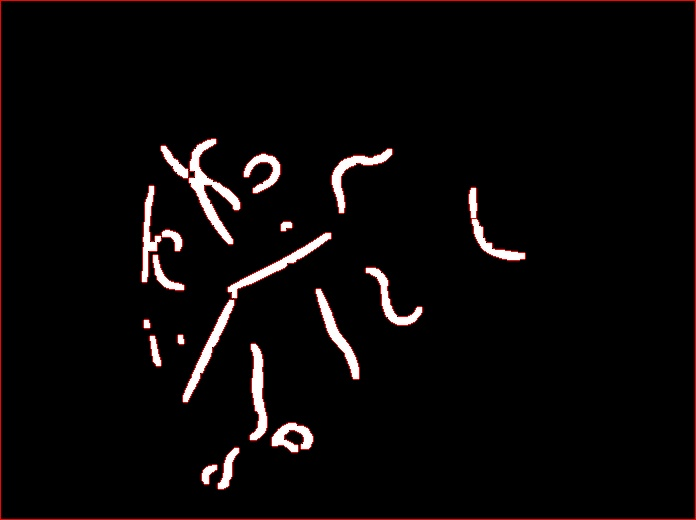
\includegraphics[width=0.9\textwidth]{A01_step2.jpg}
        \captionsetup{labelformat=empty}
        \caption{Figure 3}
    \end{subfigure}%
    \begin{subfigure}{0.5\textwidth}
        \centering
        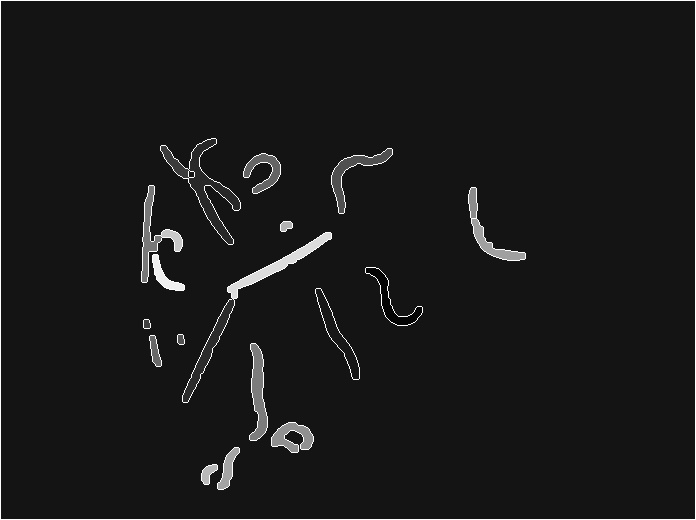
\includegraphics[width=0.9\textwidth]{A01_step2_markers.jpg}
        \captionsetup{labelformat=empty}
        \caption{Figure 4}
    \end{subfigure}
\end{figure}
\begin{figure}
    \centering
    \begin{subfigure}{0.8\textwidth}
        \centering
        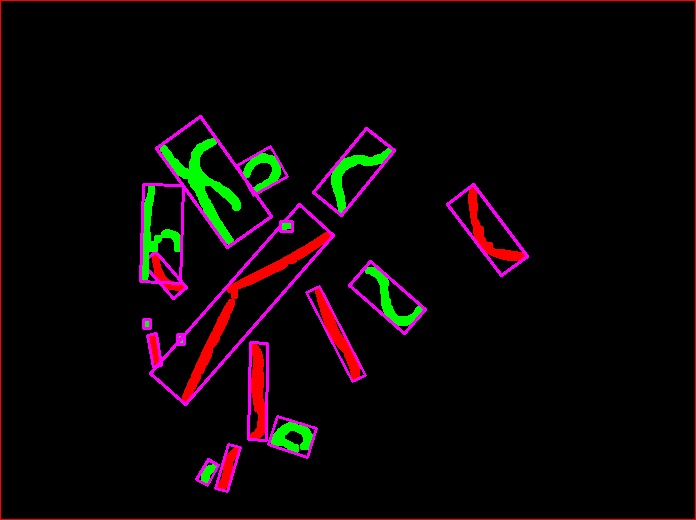
\includegraphics[width=0.8\textwidth]{A01_step3.jpg}
        \captionsetup{labelformat=empty}
        \caption{Figure 5}
    \end{subfigure}
\end{figure}

\newpage
\noindent Further results images, along with individual worms images, may be attained/updated by setting the relevant settings at the top of the script.

\section*{Fault Cases}
When a collection of worms overlap, the overlap is identified as one worm. Attempts made to identify separate worms that are touching were unsuccessful.
\\\\
If two or more worms are clustered closely but not actually touching, the script often manages to separate them, although this does depend on the size of the gaps between them.
\\\\
Finally, when thresholding, sometimes one curved worm is split into two, which will increase the worm count, and the two parts could be classified differently during dead/alive classification.

\end{document}
